\tikzstyle{basic} = [rectangle, rounded corners, minimum width=2cm, minimum height=1cm,text centered, draw=black]
\tikzstyle{arrow} = [thick,->,>=stealth]
\begin{figure}[ht]
\centering
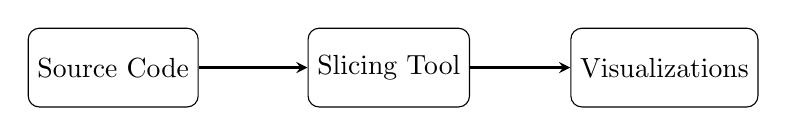
\begin{tikzpicture}[node distance=3.5cm]
\node (src) [basic] {Source Code};
\node (slice) [basic, right of=src] {Slicing Tool};
\node (viz) [basic, right of=slice] {Visualizations};

\draw [arrow] (src)--(slice);
\draw [arrow] (slice)--(viz);

\end{tikzpicture}
\caption{The flow of data in \textbf{vizSlice}}
\label{fig:dataflow}
\end{figure}
